\usetikzlibrary{positioning}
\usetikzlibrary{arrows}
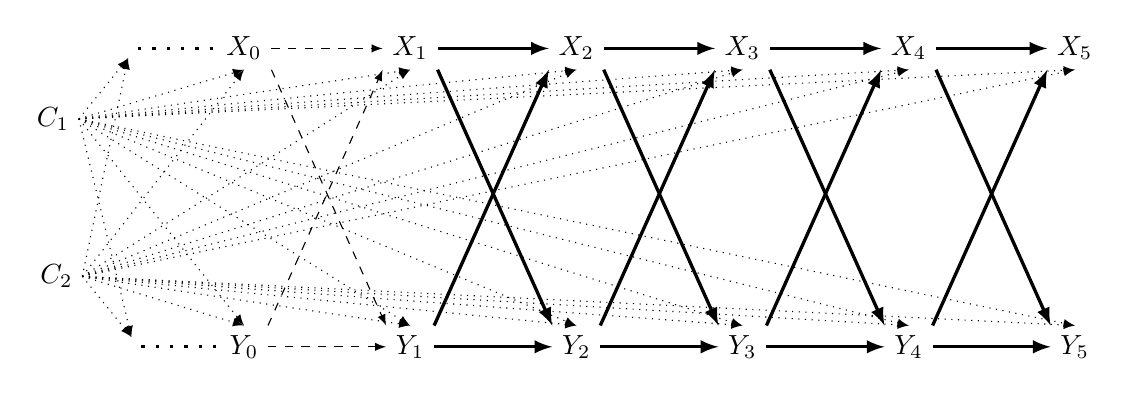
\begin{tikzpicture}[auto,node distance=.5cm, scale=0.5,
paths/.style={->, very thick, -latex},
dot/.style={dotted, ->, -latex},
double/.style={very thick, latex-latex},
dashpath/.style={dashed, ->, -latex}
]
%create nodes
\node (y1) at (0,0) {};
\node[right=1cm of y1] (yt) {$Y_0$};
\node[right=1.5cm of yt] (y2) {$Y_{1}$};
\node[right=1.5cm of y2] (y3){$Y_{2}$};
\node[right=1.5cm of y3] (y4){$Y_{3}$};
\node[right=1.5cm of y4] (y5){$Y_{4}$};
\node[right=1.5cm of y5] (y6){$Y_{5}$};

\node[above=1.5cm of yt] (ut){};
\node[above=1.5cm of y2] (u2){};
\node[above=1.5cm of y3] (u3){};
\node[above=1.5cm of y4] (u4){};
\node[above=1.5cm of y5] (u5){};
\node[above=1.5cm of y6] (u6){};

\node[above=1.5cm of ut] (xt){$X_0$};
\node[left=1cm of xt] (x1){};
\node[above=1.5cm of u2] (x2){$X_{1}$};
\node[above=1.5cm of u3] (x3){$X_{2}$};
\node[above=1.5cm of u4] (x4){$X_{3}$};
\node[above=1.5cm of u5] (x5){$X_{4}$};
\node[above=1.5cm of u6] (x6){$X_{5}$};

\node[below left=0.5cm and 0.5cm of x1] (c1){$C_{1}$};
\node[above left=0.5cm and 0.5cm of y1] (c2){$C_{2}$};

%draw paths
\draw[dashpath] (xt.south east) -- (y2.north west);
\draw[dashpath] (yt.north east) -- (x2.south west);

\draw[paths] (x2.south east) -- (y3.north west);
\draw[paths] (x3.south east) -- (y4.north west);
\draw[paths] (x4.south east) -- (y5.north west);
\draw[paths] (x5.south east) -- (y6.north west);
\draw[paths] (y2.north east) -- (x3.south west);
\draw[paths] (y3.north east) -- (x4.south west);
\draw[paths] (y4.north east) -- (x5.south west);
\draw[paths] (y5.north east) -- (x6.south west);

\draw[loosely dotted, very thick] (x1.east) -- (xt.west);
\draw[dashpath] (xt.east) -- (x2.west);
\draw[paths] (x2.east) -- (x3.west);
\draw[paths] (x3.east) -- (x4.west);
\draw[paths] (x4.east) -- (x5.west);
\draw[paths] (x5.east) -- (x6.west);
\draw[loosely dotted, very thick] (y1.east) -- (yt.west);
\draw[dashpath] (yt.east) -- (y2.west);
\draw[paths] (y2.east) -- (y3.west);
\draw[paths] (y3.east) -- (y4.west);
\draw[paths] (y4.east) -- (y5.west);
\draw[paths] (y5.east) -- (y6.west);

\draw[dot] (c1.east) -- (x1.south);
\draw[dot] (c1.east) -- (xt.south);
\draw[dot] (c1.east) -- (x2.south);
\draw[dot] (c1.east) -- (x3.south);
\draw[dot] (c1.east) -- (x4.south);
\draw[dot] (c1.east) -- (x5.south);
\draw[dot] (c1.east) -- (x6.south);

\draw[dot] (c1.east) -- (y1.north);
\draw[dot] (c1.east) -- (yt.north);
\draw[dot] (c1.east) -- (y2.north);
\draw[dot] (c1.east) -- (y3.north);
\draw[dot] (c1.east) -- (y4.north);
\draw[dot] (c1.east) -- (y5.north);
\draw[dot] (c1.east) -- (y6.north);

\draw[dot] (c2.east) -- (x1.south);
\draw[dot] (c2.east) -- (xt.south);
\draw[dot] (c2.east) -- (x2.south);
\draw[dot] (c2.east) -- (x3.south);
\draw[dot] (c2.east) -- (x4.south);
\draw[dot] (c2.east) -- (x5.south);
\draw[dot] (c2.east) -- (x6.south);

\draw[dot] (c2.east) -- (y1.north);
\draw[dot] (c2.east) -- (yt.north);
\draw[dot] (c2.east) -- (y2.north);
\draw[dot] (c2.east) -- (y3.north);
\draw[dot] (c2.east) -- (y4.north);
\draw[dot] (c2.east) -- (y5.north);
\draw[dot] (c2.east) -- (y6.north);

\end{tikzpicture}